\documentclass{article}

\usepackage{listings}
\usepackage{fancyhdr}
\usepackage{extramarks}
\usepackage{amsmath}
\usepackage{amsthm}
\usepackage{amsfonts}
\usepackage{tikz}
\usepackage[plain]{algorithm}
\usepackage{algpseudocode}
\usetikzlibrary{automata,positioning}

\usepackage{xcolor}

\definecolor{codegreen}{rgb}{0,0.6,0}
\definecolor{codegray}{rgb}{0.5,0.5,0.5}
\definecolor{codepurple}{rgb}{0.58,0,0.82}
\definecolor{backcolour}{rgb}{0.95,0.95,0.92}

\lstdefinestyle{mystyle}{
	backgroundcolor=\color{backcolour},   
	commentstyle=\color{codegreen},
	keywordstyle=\color{magenta},
	numberstyle=\tiny\color{codegray},
	stringstyle=\color{codepurple},
	basicstyle=\ttfamily\footnotesize,
	breakatwhitespace=false,         
	breaklines=true,                 
	captionpos=b,                    
	keepspaces=true,                 
	numbers=left,                    
	numbersep=5pt,                  
	showspaces=false,                
	showstringspaces=false,
	showtabs=false,                  
	tabsize=2
}

\lstset{style=mystyle}

%
% Basic Document Settings
%

\topmargin=-0.45in
\evensidemargin=0in
\oddsidemargin=0in
\textwidth=6.5in
\textheight=9.0in
\headsep=0.25in

\linespread{1.1}

\pagestyle{fancy}
\lhead{\hmwkAuthorName}
\chead{\hmwkClass\ (\hmwkClassInstructor\ \hmwkClassTime): \hmwkTitle}
\rhead{\firstxmark}
\lfoot{\lastxmark}
\cfoot{\thepage}

\renewcommand\headrulewidth{0.4pt}
\renewcommand\footrulewidth{0.4pt}

\setlength\parindent{0pt}

%
% Create Problem Sections
%

\newcommand{\enterProblemHeader}[1]{
    \nobreak\extramarks{}{Problem \arabic{#1} continued on next page\ldots}\nobreak{}
    \nobreak\extramarks{Problem \arabic{#1} (continued)}{Problem \arabic{#1} continued on next page\ldots}\nobreak{}
}

\newcommand{\exitProblemHeader}[1]{
    \nobreak\extramarks{Problem \arabic{#1} (continued)}{Problem \arabic{#1} continued on next page\ldots}\nobreak{}
    \stepcounter{#1}
    \nobreak\extramarks{Problem \arabic{#1}}{}\nobreak{}
}

\setcounter{secnumdepth}{0}
\newcounter{partCounter}
\newcounter{homeworkProblemCounter}
\setcounter{homeworkProblemCounter}{1}
\nobreak\extramarks{Problem \arabic{homeworkProblemCounter}}{}\nobreak{}

%
% Homework Problem Environment
%
% This environment takes an optional argument. When given, it will adjust the
% problem counter. This is useful for when the problems given for your
% assignment aren't sequential. See the last 3 problems of this template for an
% example.
%
\newenvironment{homeworkProblem}[1][-1]{
    \ifnum#1>0
        \setcounter{homeworkProblemCounter}{#1}
    \fi
    \section{Problem \arabic{homeworkProblemCounter}}
    \setcounter{partCounter}{1}
    \enterProblemHeader{homeworkProblemCounter}
}{
    \exitProblemHeader{homeworkProblemCounter}
}

%
% Homework Details
%   - Title
%   - Due date
%   - Class
%   - Section/Time
%   - Instructor
%   - Author
%

\newcommand{\hmwkTitle}{Homework 3 CI}
\newcommand{\hmwkDueDate}{Feburary 26, 2020}
\newcommand{\hmwkClass}{Phys 216}
\newcommand{\hmwkClassTime}{Section 509}
\newcommand{\hmwkClassInstructor}{Professor Dr. O}
\newcommand{\hmwkAuthorName}{\textbf{Amari West}}
\newcommand{\hmwkDueTime}{11:59pm \\ 18 Pages}

%
% Title Page
%

\title{
    \vspace{2in}
    \textmd{\textbf{\hmwkClass:\ \hmwkTitle}}\\
    \normalsize\vspace{0.1in}\small{Due\ on\ \hmwkDueDate\ at \hmwkDueTime}\\
    \vspace{0.1in}\large{\textit{\hmwkClassInstructor\ \hmwkClassTime}}
    \vspace{3in}
}

\author{\hmwkAuthorName}
\date{}

\renewcommand{\part}[1]{\textbf{\large Part \Alph{partCounter}}\stepcounter{partCounter}\\}

%
% Various Helper Commands
%

% Useful for algorithms
\newcommand{\alg}[1]{\textsc{\bfseries \footnotesize #1}}

% For derivatives
\newcommand{\deriv}[1]{\frac{\mathrm{d}}{\mathrm{d}x} (#1)}

% For partial derivatives
\newcommand{\pderiv}[2]{\frac{\partial}{\partial #1} (#2)}

% Integral dx
\newcommand{\dx}{\mathrm{d}x}

% Alias for the Solution section header
\newcommand{\solution}{\textbf{\large Solution}}

% Probability commands: Expectation, Variance, Covariance, Bias
\newcommand{\E}{\mathrm{E}}
\newcommand{\Var}{\mathrm{Var}}
\newcommand{\Cov}{\mathrm{Cov}}
\newcommand{\Bias}{\mathrm{Bias}}

% Allow double underline
\def\doubleunderline#1{\underline{\underline{#1}}}

% Allow for units in math mode
\newcommand{\unit}[1]{\ensuremath{\, \mathrm{#1}}}

\begin{document}

\maketitle

\pagebreak

\begin{homeworkProblem}
	For a normal population with known variance $\sigma^2$, what is the confidence level for the CI
	
	\[
		\bar{x} - \frac{2.14\sigma}{\sqrt{n}} \leq \mu \leq \bar{x} + \frac{2.14\sigma}{\sqrt{n}}
	\]
	
	\textbf{\underline{Given}}
	\\
	
	\begin{itemize}
		\item $\sigma^2$ is known.
		\item The given $z$-values are -2.14 and 2.14.
	\end{itemize}
	
	\textbf{\underline{Find}}
	\\
	
	\begin{itemize}
		\item The confidence level for the interval
	\end{itemize}
	
	\textbf{\underline{Diagram}}
	
	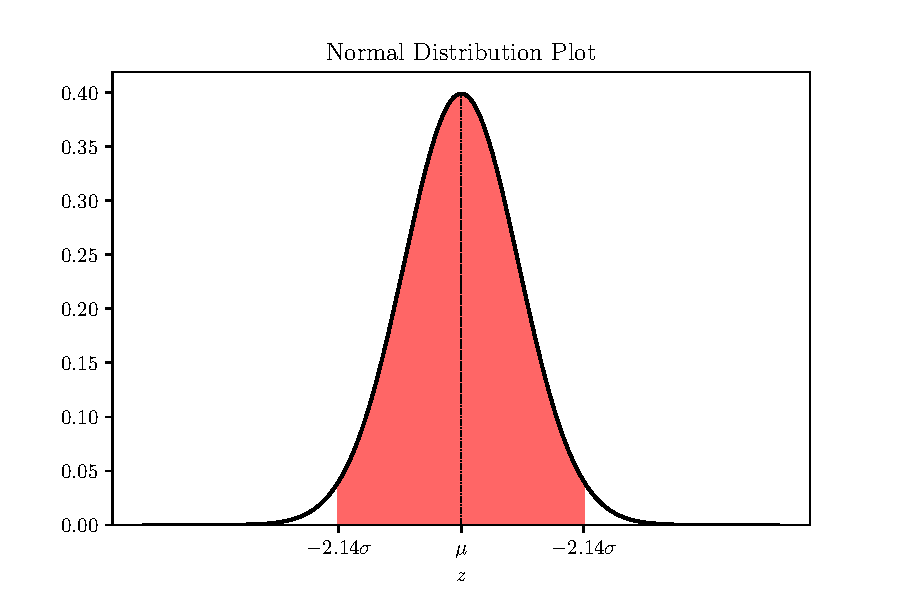
\includegraphics[scale=0.9]{problem1}
	
	\textbf{\underline{Theory}}
	\\
	
	The confidence level for the CI is found by using the value given as a coefficient of $\sigma$ and using it to find the $p$-value. With that, the smaller $p$-value is subtracted from the larger $p$-value and the difference multiplied by 100\% becomes the answer. 
	\[
	P(L \leq \mu \leq U) = \frac{P}{100\%}
	\] 
	
	\textbf{\underline{Assumption}}
	\\
	
	The data follows a normal distribution of $N(\mu, (\sigma)^2)$
	\\
	
	\pagebreak
	
	\textbf{\underline{Solution}}
	\\
	
	To find the confidence level, first find the $p$-value and plug in given variables into the following equation.
	
	\[
	\begin{split}
		\frac{P}{100\%} &= P(L \leq \mu \leq U)
		\\
		&= P(-2.14 \leq \mu \leq 2.14)
		\\
		&= 0.9838 - 0.0162
		\\
		&= 0.9676
	\end{split}
	\]
	
	Now, multiply both sides by 100\%.
	
	\[
	\begin{split}
		P = \doubleunderline{96.76\%}
	\end{split}
	\]
	
	\textbf{\underline{Conclusion}}
	\\
	
	The confidence level for the interval is \boxed{96.76\%.}
	
\end{homeworkProblem}

\pagebreak

\begin{homeworkProblem}
	An electrical firm manufactures light bulbs that have a length of life that is approximately normally
	distributed with a standard deviation of 40 hours. If a sample of 30 bulbs has an average life of 780
	hours, find a 96\% confidence interval for the population mean of all bulbs produced by this firm.
	\\	
	
	\textbf{\underline{Given}}
	\\
	
	\begin{itemize}
		\item $\sigma$ = 40 hours
		\item $N$ = 30 bulbs
		\item $\mu$ = 780 hours
		\item $P$ = 0.96
	\end{itemize}
	
	\textbf{\underline{Find}}
	\\
	
	\begin{itemize}
		\item The upper and lower bound of the interval.
	\end{itemize}
	
	\textbf{\underline{Diagram}}
	\\
	
	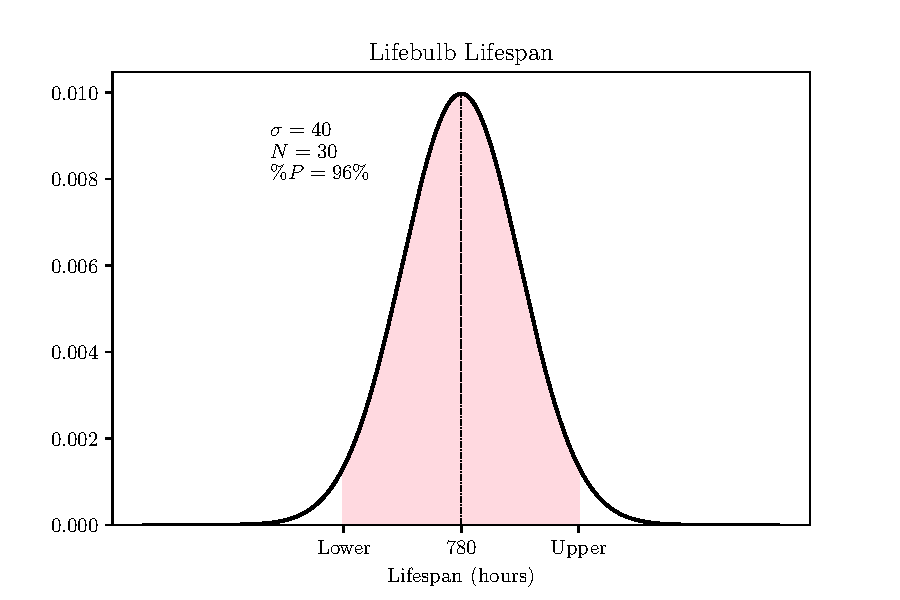
\includegraphics[scale=0.9]{problem2}
	
	\textbf{\underline{Theory}}
	\\
	
	To find the upper and lower bound of the interval with the acceptable confidence level, all known values need to be plugged into the following equations.
	
	\[
	\begin{split}
		P(L \leq \mu \leq U) &= \bar{x} - z_\frac{\alpha}{2} \frac{\sigma}{\sqrt{n}} \leq \mu \leq \bar{x} + z_\frac{\alpha}{2} \frac{\sigma}{\sqrt{n}}
	\end{split}
	\]
	
	\textbf{\underline{Assumption}}
	\\
	
	The data follows the normal distribution curve $N(780, (40)^2)$
	\\
	
	\textbf{\underline{Solution}}
	\\
	
	Note: Python and JupyterNotebooks were used to compute the answer. Among the modules used were \verb|scipy.stats|, \verb|numpy|, and \verb|sympy|.
	\\
	
	\verb|Input:|
	
	\begin{lstlisting}[language=Python]
	from scipy.stats import norm
	import numpy as np
	from sympy import *
	from IPython.display import *
	import ipywidgets as widgets
	import math as m
	
	def output(input):
	return display(Latex(input))
	
	def equ(input):
	equation = ' $' + latex(input) + '$ '
	return equation
	
	x_lower = widgets.FloatText() # Unknown
	x_upper = widgets.FloatText() # Unknown
	mu = widgets.FloatText() # mu = 780
	sigma = widgets.FloatText(value=1) # sigma = 40
	num = widgets.FloatText(value=1) # num = 30
	p = widgets.FloatText() # p = .96
	
	alpha = 1 - p.value
	half_alpha = alpha / 2
	
	z_alpha = abs(norm.ppf(half_alpha))
	
	upper = mu.value + z_alpha * (sigma.value / m.sqrt(num.value))
	lower = mu.value - z_alpha * (sigma.value / m.sqrt(num.value))
	
	output('The upper estimate of $\mu$ is' + equ(upper))
	output('The lower estimate of $\mu$ is' + equ(lower))
	\end{lstlisting}
	
	\verb|Output:|
	
	\begin{lstlisting}
	The upper estimate of mu is 794.9984614107295
	The lower estimate of mu is 765.0015385892705
	\end{lstlisting}
	
	\textbf{\underline{Conclusion}}
	\\
	
	The interval with a confidence level of 96\% has a lower bound of \boxed{795} and an upper bound of \boxed{765.}
	
\end{homeworkProblem}

\pagebreak

\begin{homeworkProblem}
	You are working part-time at a road construction firm. Your boss knows you are learning some statistics in your classes this semester and calls you into the office. He says, “We’ve taken sample densities from loads of asphalt we’ve gotten from our supplier. The information from their company says their process produces a consistent density with a standard deviation of 2.65 pounds per cubic foot. Here’s the data we’ve collected (see file “CIData.txt”). Can you give me an estimate of the average density that our supplier’s process is producing? I want to be 80\% confident of the range you provide.” Download the data file “CIData.txt”. Use Python or Excel to calculate the sample average (please include one decimal place). You also need to know the number of measurements in the sample.
	\\
	
	
	\textbf{\underline{Given}}
	\\
	\begin{itemize}
		\item $\sigma$ = 2.65
		\item $\bar{x}$ = 145.8
		\item $N$ = 46
		\item $P$ = 0.80
	\end{itemize}
	
	\textbf{\underline{Find}}
	\\
		\begin{itemize}
		\item A range of the average that has an 80\% confidence level.
	\end{itemize}
	
	\textbf{\underline{Diagram}}
	\\
	
	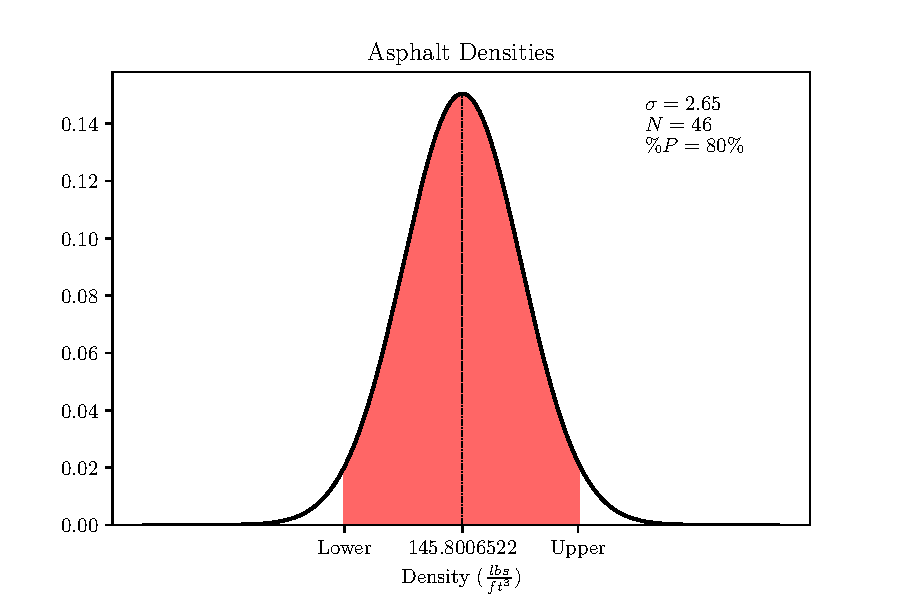
\includegraphics[scale=0.9]{problem3}
	
	
	\textbf{\underline{Theory}}
	\\
	
	To find the upper and lower bound of the interval with the acceptable confidence level, all known values need to be plugged into the following equations.
	
	\[
	\begin{split}
	P(L \leq \mu \leq U) &= \bar{x} - z_\frac{\alpha}{2} \frac{\sigma}{\sqrt{n}} \leq \mu \leq \bar{x} + z_\frac{\alpha}{2} \frac{\sigma}{\sqrt{n}}
	\end{split}
	\]
	
	\textbf{\underline{Assumption}}
	\\
	
	The data follows the normal distribution curve $N(145.8, (2.65)^2)$
	\\
	
	\textbf{\underline{Solution}}
	\\
	
		Note: Python and JupyterNotebooks were used to compute the answer. Among the modules used were \verb|scipy.stats|, \verb|numpy|, and \verb|sympy|.
	\\
	
	\verb|Input:|
	
	\begin{lstlisting}[language=Python]
	from scipy.stats import norm
	import numpy as np
	from sympy import *
	from IPython.display import *
	import ipywidgets as widgets
	import math as m
	
	def output(input):
	return display(Latex(input))
	
	def equ(input):
	equation = ' $' + latex(input) + '$ '
	return equation
	
	x_lower = widgets.FloatText() # Unknown
	x_upper = widgets.FloatText() # Unknown
	mu = widgets.FloatText() # mu = 145.8
	sigma = widgets.FloatText(value=1) # sigma = 2.65
	num = widgets.FloatText(value=1) # num = 46
	p = widgets.FloatText() # p = .80
	
	alpha = 1 - p.value
	half_alpha = alpha / 2
	
	z_alpha = abs(norm.ppf(half_alpha))
	
	upper = mu.value + z_alpha * (sigma.value / m.sqrt(num.value))
	lower = mu.value - z_alpha * (sigma.value / m.sqrt(num.value))
	
	output('The upper estimate of $\mu$ is' + equ(upper))
	output('The lower estimate of $\mu$ is' + equ(lower))
	\end{lstlisting}
	
	\verb|Output:|
	
	\begin{lstlisting}
	The upper estimate of mu is 146.30072934480376
	The lower estimate of mu is 145.29927065519627
	\end{lstlisting}
	
	\textbf{\underline{Conclusion}}
	\\
	
	The interval with a confidence level of 80\% has a lower bound of \boxed{146.3} and an upper bound of \boxed{145.3.}
\end{homeworkProblem}

\pagebreak

\begin{homeworkProblem}
	A civil engineer is analyzing the compressive strength of concrete. Compressive strength is
	approximately normally distributed with variance $\sigma^2$ = 1000 psi$^2$ A random sample of 12 specimens has a mean compressive strength of $\bar{x}$ = 3255.42 psi.
	a) Construct a 95\% two-sided CI on mean compressive strength.
	b) Construct a 99\% two-sided CI on mean compressive strength.
	c) Compare the width of the 99\% CI with the width of the 95\% CI: evaluate the ratio $\frac{99\% Cl}{95\% Cl}$ 
	\\
	
	\textbf{\underline{Given}}
	\\
	
	\begin{itemize}
		\item $\sigma^2$ = 1000 psi$^2$
		\item $N$ = 12
		\item $\bar{x}$ = 3255.45 psi
	\end{itemize}
	
	\textbf{\underline{Find}}
	\\
	
	\begin{itemize}
		\item A 95\% two-sided CI on mean compressive strength.
		\item A 99\% two-sided CI on mean compressive strength.
		\item The ratio of the widths of part A and part B
	\end{itemize}
	
	\textbf{\underline{Diagram}}
	\\
	
	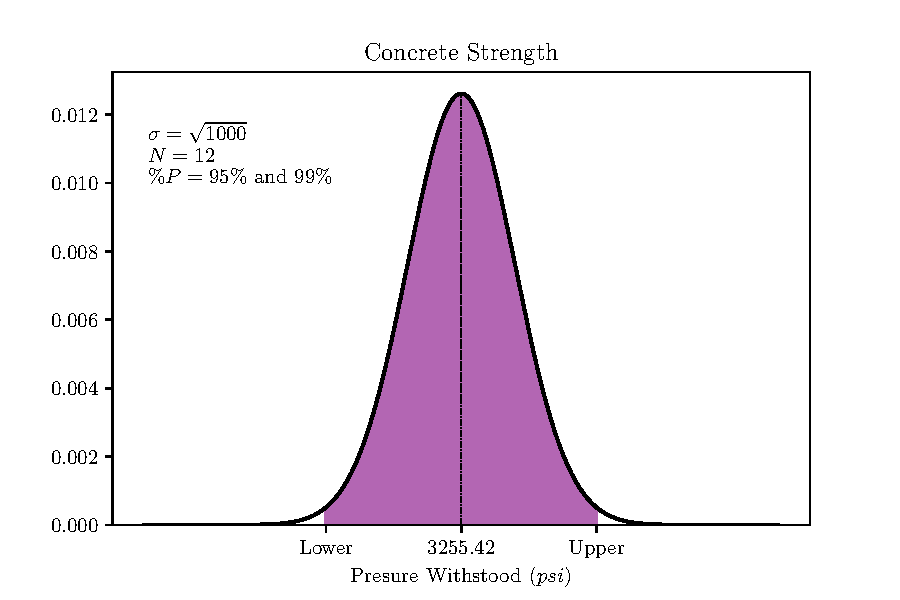
\includegraphics[scale=0.9]{problem4}
	
	\textbf{\underline{Theory}}
	\\
	
	To find the upper and lower bound of the interval with the acceptable confidence level, all known values need to be plugged into the following equations.
	
	\[
	\begin{split}
	P(L \leq \mu \leq U) &= \bar{x} - z_\frac{\alpha}{2} \frac{\sigma}{\sqrt{n}} \leq \mu \leq \bar{x} + z_\frac{\alpha}{2} \frac{\sigma}{\sqrt{n}}
	\end{split}
	\]
	
	\textbf{\underline{Assumption}}
	\\
	
	The data follows the normal distribution curve $N(3255.45, 1000)$
	\\	
	
	\textbf{\underline{Solution}}
	\\

	Note: Python and JupyterNotebooks were used to compute the answer. Among the modules used were \verb|scipy.stats|, \verb|numpy|, and \verb|sympy|.
	\\
	
	\textbf{Part A}
	
	\verb|Input:|
	
	\begin{lstlisting}[language=Python]
	from scipy.stats import norm
	import numpy as np
	from sympy import *
	from IPython.display import *
	import ipywidgets as widgets
	import math as m
	
	def output(input):
	return display(Latex(input))
	
	def equ(input):
	equation = ' $' + latex(input) + '$ '
	return equation
	
	x_lower = widgets.FloatText() # Unknown
	x_upper = widgets.FloatText() # Unknown
	mu = widgets.FloatText() # mu = 3255.42
	sigma = widgets.FloatText(value=1) # sigma = sqrt(1000)
	num = widgets.FloatText(value=1) # num = 12
	p = widgets.FloatText() # p = .95
	
	alpha = 1 - p.value
	half_alpha = alpha / 2
	
	z_alpha = abs(norm.ppf(half_alpha))
	
	upper = mu.value + z_alpha * (sigma.value / m.sqrt(num.value))
	lower = mu.value - z_alpha * (sigma.value / m.sqrt(num.value))
	
	output('The upper estimate of $\mu$ is' + equ(upper))
	output('The lower estimate of $\mu$ is' + equ(lower))
	\end{lstlisting}
	
	\verb|Output:|
	
	\begin{lstlisting}
	The upper estimate of mu is 3273.311941437181
	The lower estimate of mu is 3237.5280585628193
	\end{lstlisting}
	
	\pagebreak
	
	\textbf{Part B}
	
	\verb|Input:|
	
	\begin{lstlisting}[language=Python]
	from scipy.stats import norm
	import numpy as np
	from sympy import *
	from IPython.display import *
	import ipywidgets as widgets
	import math as m
	
	def output(input):
	return display(Latex(input))
	
	def equ(input):
	equation = ' $' + latex(input) + '$ '
	return equation
	
	x_lower = widgets.FloatText() # Unknown
	x_upper = widgets.FloatText() # Unknown
	mu = widgets.FloatText() # mu = 3255.42
	sigma = widgets.FloatText(value=1) # sigma = sqrt(1000)
	num = widgets.FloatText(value=1) # num = 12
	p = widgets.FloatText() # p = .99
	
	alpha = 1 - p.value
	half_alpha = alpha / 2
	
	z_alpha = abs(norm.ppf(half_alpha))
	
	upper = mu.value + z_alpha * (sigma.value / m.sqrt(num.value))
	lower = mu.value - z_alpha * (sigma.value / m.sqrt(num.value))
	
	output('The upper estimate of $\mu$ is' + equ(upper))
	output('The lower estimate of $\mu$ is' + equ(lower))
	\end{lstlisting}
	
	\verb|Output:|
	
	\begin{lstlisting}
	The upper estimate of mu is 3278.933996897288
	The lower estimate of mu is 3231.906003102712
	\end{lstlisting}
	
	\textbf{Part C}
	\\
	The ratio evaluation was done by hand. First, the difference between the upper and lower bounds were found for both ranges.
	\\
	
	From part A...
	\[
	\begin{split}
		(U - L) &= 3273.31 - 3237.53
		\\
		&= 35.78
	\end{split}
	\]
	
	From part B...
	\[
	\begin{split}
		(U - L) &= 3278.93 - 3231.91)
		\\
		&= 47.02
	\end{split}
	\]
	
	Now, the ratio is evaluated.
	\[
	\begin{split}
		\frac{47.02}{35.78} &= \doubleunderline{1.314}
	\end{split}
	\]
	\textbf{\underline{Conclusion}}
	\\
	
	For Part A, the interval with a confidence level of 95\% has a lower bound of \boxed{3237.53} and an upper bound of \boxed{3273.31.}
	\\
	
	For Part B, the interval with a confidence level of 95\% has a lower bound of \boxed{3231.91} and an upper bound of \boxed{3278.93.}
	\\
	
	The ratio between the two ranges is \boxed{1.314.}
\end{homeworkProblem}

\pagebreak

\begin{homeworkProblem}
	
	In a random sample of 80 teenagers, the average number of texts handled in a day is 50. The 96\%
	confidence interval for the mean number of texts handled by teens daily is given as 46 to 54.
	a) Find the value of standard deviation $\sigma$ that was used to calculate this CI.
	b) If the number of participants per sample were doubled, by what factor would the confidence
	interval change (keeping the same confidence level)? Evaluate width of 96\% CI from part b) over width of 96\% CI from part a)
	\\
	
	\textbf{\underline{Given}}
	\\
	
	\begin{itemize}
		\item $N$ = 80
		\item $\bar{x}$ = 50
		\item $P$ = 0.96
		\item Lower Bound = 46
		\item Upper Bound = 54
	\end{itemize}
	
	\textbf{\underline{Find}}
	\\
	
	\begin{itemize}
		\item The standard deviation.
		\item The factor at which the confidence interval would change if the sample doubled.
	\end{itemize}
	
	\textbf{\underline{Diagram}}
	\\
	
	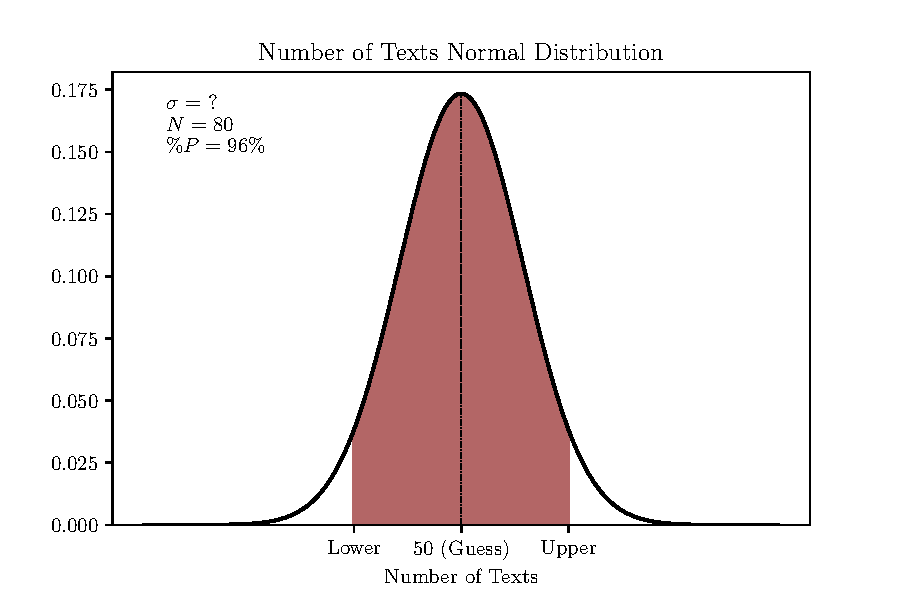
\includegraphics[scale=0.9]{problem5}
	
	\textbf{\underline{Theory}}
	\\
	
	To find the upper and lower bound of the interval with the acceptable confidence level, all known values need to be plugged into the following equations.
	
	\[
	\begin{split}
	P(L \leq \mu \leq U) &= \bar{x} - z_\frac{\alpha}{2} \frac{\sigma}{\sqrt{n}} \leq \mu \leq \bar{x} + z_\frac{\alpha}{2} \frac{\sigma}{\sqrt{n}}
	\end{split}
	\]
	
	\textbf{\underline{Assumption}}
	\\
	
	The data follows a normal distribution.
	\\
	
	\textbf{\underline{Solution}}
	\\
	
	\textbf{Part A}
	\\
	
	Note: Python and JupyterNotebooks were used to compute the answer. Among the modules used were \verb|scipy.stats|, \verb|numpy|, and \verb|sympy|.
	\\
	
	\verb|Input:|
	
	\begin{lstlisting}[language=Python]
	from scipy.stats import norm
	import numpy as np
	from sympy import *
	from IPython.display import *
	import ipywidgets as widgets
	import math as m
	
	def output(input):
	return display(Latex(input))
	
	def equ(input):
	equation = ' $' + latex(input) + '$ '
	return equation
	
	x_lower = widgets.FloatText() # L = 46
	x_upper = widgets.FloatText() # U = 54
	mu = widgets.FloatText() # mu = 50
	sigma = widgets.FloatText(value=1) # sigma = unknown
	num = widgets.FloatText(value=1) # num = 80
	p = widgets.FloatText() # p = .96
	
	alpha = 1 - p.value
	half_alpha = alpha / 2

	z_alpha = norm.ppf(half_alpha)

	sigma_x = (x_lower.value - mu.value) * m.sqrt(num.value) / z_alpha

	output('The value of sigma is' + equ(sigma_x))
	\end{lstlisting}
	
	\verb|Output:|
	
	\begin{lstlisting}
	The value of sigma is 17.420380580501465
	\end{lstlisting}
	
	\pagebreak
	
	\textbf{Part B}
	\\
	
	Note: Python and JupyterNotebooks were used to compute the answer. Among the modules used were \verb|scipy.stats|, \verb|numpy|, and \verb|sympy|.
	\\
	
	\verb|Input:|
	
	\begin{lstlisting}[language=Python]
	from scipy.stats import norm
	import numpy as np
	from sympy import *
	from IPython.display import *
	import ipywidgets as widgets
	import math as m
	
	def output(input):
	return display(Latex(input))
	
	def equ(input):
	equation = ' $' + latex(input) + '$ '
	return equation
	
	x_lower = widgets.FloatText() # L = unknown
	x_upper = widgets.FloatText() # U = unknown
	mu = widgets.FloatText() # mu = 50
	sigma = widgets.FloatText(value=1) # sigma = 17
	num = widgets.FloatText(value=1) # num = 160
	p = widgets.FloatText() # p = .96
	
	alpha = 1 - p.value
	half_alpha = alpha / 2

	z_alpha = abs(norm.ppf(half_alpha))

	upper = mu.value + z_alpha * (sigma.value / m.sqrt(num.value))
	lower = mu.value - z_alpha * (sigma.value / m.sqrt(num.value))

	output('The upper estimate of $\mu$ is' + equ(upper))
	output('The lower estimate of $\mu$ is' + equ(lower))
	\end{lstlisting}
	
	\verb|Output:|
	
	\begin{lstlisting}
	The upper estimate of mu is 52.82836533251332
	The lower estimate of mu is 47.17163466748668
	\end{lstlisting}
	
	From part A...
	\[
	\begin{split}
	(U - L) &= 54 - 46
	\\
	&= 8
	\end{split}
	\]
	
	From part B...
	\[
	\begin{split}
	(U - L) &= 53 - 47
	\\
	&= 6
	\end{split}
	\]
	
	Now, the ratio is evaluated.
	\[
	\begin{split}
	\frac{6}{8} &= \doubleunderline{0.75}
	\end{split}
	\]
	
	
	\textbf{\underline{Conclusion}}
	\\
	Since only a whole number of texts can be sent, all answers will be expressed with whole numbers. The value of $\sigma$ is \boxed{17}. When the sample size is doubled, the lower bound is \boxed{47} and the upper bound is \boxed{53.} The ratio between these ranges is \boxed{0.75}
	
\end{homeworkProblem}

\pagebreak

\begin{homeworkProblem}
	Hotel managers wish to learn the average length of stay of all visitors that are senior citizens. A
	statistician determines that for a 90\% confidence level estimate of the average length of stay to within
	$\pm$ 1.5 days, 65 senior visitors’ check-in/check-out records will have to be examined. How many
	records should be looked at to obtain a 90\% confidence level estimate to within $\pm$ 0.5 days?
	\\
	
	\textbf{\underline{Given}}
	\\
	
	\begin{itemize}
		\item $P$ = 0.90
		\item The intervals at which the confidence level is recorded
		\item The original sample size is 65
	\end{itemize}
	
	\textbf{\underline{Find}}
	\\
	
	\begin{itemize}
		\item $\sigma$ needs to be found to find the final answer.
		\item The number of data points to establish a 90\% confidence level with 0.5 days
	\end{itemize}
	
	\textbf{\underline{Diagram}}
	\\
	
	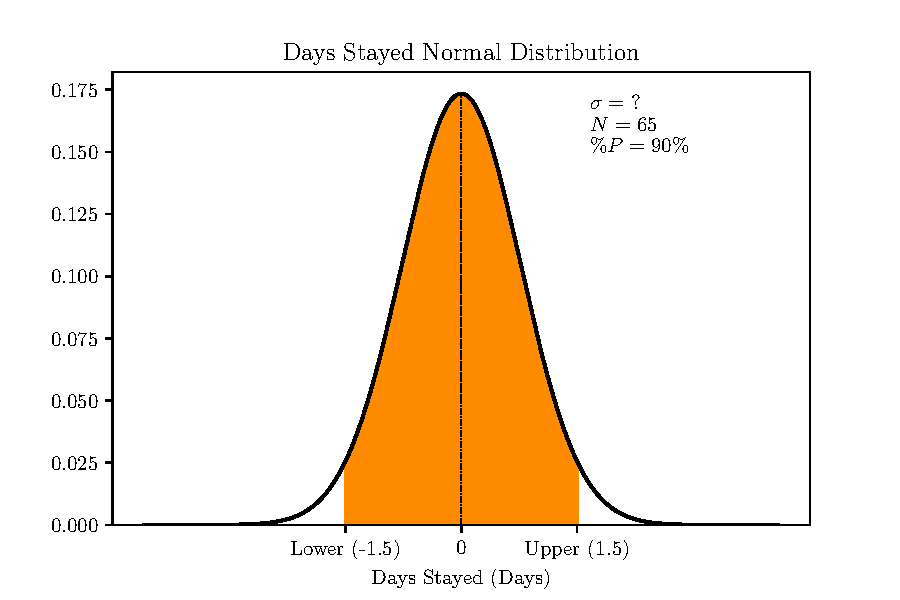
\includegraphics[scale=0.9]{problem6}
	
	\textbf{\underline{Theory}}
	\\
	
	To find the upper and lower bound of the interval with the acceptable confidence level, all known values need to be plugged into the following equations.
	
	\[
	\begin{split}
	P(L \leq \mu \leq U) &= \bar{x} - z_\frac{\alpha}{2} \frac{\sigma}{\sqrt{n}} \leq \mu \leq \bar{x} + z_\frac{\alpha}{2} \frac{\sigma}{\sqrt{n}}
	\end{split}
	\]
	
	\textbf{\underline{Assumption}}
	\\
	
	The data follows the normal distribution curve $N(0, (\sigma))$
	\\	
	
	\textbf{\underline{Solution}}
	\\
	
	First, $\sigma$ must be found.
	
	Note: Python and JupyterNotebooks were used to compute the answer. Among the modules used were \verb|scipy.stats|, \verb|numpy|, and \verb|sympy|.
	\\
	
	\verb|Input:|
	
	\begin{lstlisting}[language=Python]
	from scipy.stats import norm
	import numpy as np
	from sympy import *
	from IPython.display import *
	import ipywidgets as widgets
	import math as m
	
	def output(input):
	return display(Latex(input))
	
	def equ(input):
	equation = ' $' + latex(input) + '$ '
	return equation
	
	x_lower = widgets.FloatText() # L = -1.5
	x_upper = widgets.FloatText() # U = 1.5
	mu = widgets.FloatText() # mu = 0
	sigma = widgets.FloatText(value=1) # sigma = unknown
	num = widgets.FloatText(value=1) # num = 65
	p = widgets.FloatText() # p = .90
	
	alpha = 1 - p.value
	half_alpha = alpha / 2
	
	z_alpha = norm.ppf(half_alpha)
	
	sigma_x = (x_lower.value - mu.value) * m.sqrt(num.value) / z_alpha
	
	output('The value of sigma is' + equ(sigma_x))
	\end{lstlisting}
	
	\verb|Output:|
	
	\begin{lstlisting}
	The value of sigma is 7.352257018067546
	\end{lstlisting}
	
	Now, find the number of samples required to have a 90\% confidence estimate in a $\pm 0.5$ days. 
	\\
	
	\verb|Input:|
	
	\begin{lstlisting}[language=Python]
	from scipy.stats import norm
	import numpy as np
	from sympy import *
	from IPython.display import *
	import ipywidgets as widgets
	import math as m
	
	def output(input):
	return display(Latex(input))
	
	def equ(input):
	equation = ' $' + latex(input) + '$ '
	return equation
	
	x_lower = widgets.FloatText() # L = -0.5
	x_upper = widgets.FloatText() # U = 0.5
	mu = widgets.FloatText() # mu = 0
	sigma = widgets.FloatText(value=1) # sigma = 7.352257018067546
	num = widgets.FloatText(value=1) # num = unknown
	p = widgets.FloatText() # p = .90
	
	alpha = 1 - p.value
	half_alpha = alpha / 2
	
	z_alpha = norm.ppf(half_alpha)
	
	num_x = ((sigma.value * z_alpha)/(x_upper.value - mu.value)) ** 2
	
	output('The sample number is' + equ(num_x))
	\end{lstlisting}
	
	\verb|Output:|
	\\
	
	\begin{lstlisting}
	The sample number is 584.9999999999999
	\end{lstlisting}
	
	
	
	\textbf{\underline{Conclusion}}
	\\
	
	At least \boxed{585} records should be looked at to obtain a 90\% confidence level estimate with $\pm 0.5$ days.
\end{homeworkProblem}



\end{document}
